\chapter{Protein Folding}

\say{\textit{la forma è l'immagine plastica	della funzione}}\footnote{\fullcite{ruffini1925fisiogenia}}\\

La correlazione tra forma e funzione si rivela fondamentale nel caso delle proteine. Un canale ionico neuronale permette il passaggio di ioni grazie alla sua forma a canale; una ferritina cattura e immagazzina gli ioni ferro grazie alla sua forma a sfera cava. 

\par Il ripiegamento delle proteine (\textit{protein folding}) è il processo di ripiegamento molecolare attraverso il quale le proteine ottengono la loro struttura tridimensionale che permette loro di svolgere la loro funzione biologica. Il ripiegamento avviene sia contemporaneamente alla sintesi proteica nei ribosomi sia al termine di questa.

\par La prima teoria del ripiegamento proteico è stata proposta negli anni trenta del 20° secolo da Hsien Wu\supercite{wu1931studies}, legata al processo di denaturazione.  

\par robe \\


--- Biochemists now know the amino acid sequence for about
160 million proteins, with about 4.5–5 million added each
month, and the three-dimensional shape for about 40,000.
Researchers have tried to correlate the primary structure of
many proteins with their three-dimensional structure to dis-
cover the rules of protein folding. Unfortunately, however,
the protein-folding process is not that simple. Most proteins
probably go through several intermediate structures on their
way to a stable shape, and looking at the mature structure
does not reveal the stages of folding required to achieve that
form

Cos'è stu cazz e protein folding?

• cos’è il problema del protein folding: non solo la struttura finale\\
• 3 sottoproblemi: folding code, protein structure prediction e folding process\\
• le domande di principio del protein folding\\
• struttura delle proteine (4 livelli)\\
• Domini, Residui, Motivi, Giri\\
• postulato di Anfinsen, paradosso di Levinthal\\
• interazioni (covalenti, polari, van der Waals, ..)\\
• una forza dominante o tante piccole forze?\\
• Cambio di paradigma da metà anni ‘80\\
• chaperonine, sintesi\\
• misfolding (denaturazione)\\
• struttura e funzione, malattie e prioni\\
• Limiti al ripiegamento: angoli di tersione e piano di Ramachandran\\
• processo spontaneo: energia di Gibbs, entalpia, entropia\\


[ soft computing articolo]
-- strutture --
pri-
mary structure of proteins consist of linear sequences of twenty
natural amino acids joined together by peptide bonds. The sec-
ondary structure of a protein refers to the interactions due to
a regular arrangement of hydrogen bonds between CO and NH
groups (carboxyl and amino) of its amino acids, forming different
motifs ( ̨-helix, ˇ-sheet, loops and turns). The tertiary structure is
a description of the complex and irregular folding of the polypep-
tide chain in three dimensions. These complex structures are held
together by a combination of several molecular interactions (e.g.
ionic, hydrophobic or hydrogen bonds) that involve the amino acids
of the chain. The quaternary structure is the final dimensional struc-
ture formed by all the polypeptide chains making up a protein [13].

---- native state  ---
A protein spontaneously folds into a 3-dimensional structure
after having been manufactured in the ribosomes. A specific pro-
tein will fold in the same way and will end up with the same 3D
structure. This phenomenon is called the native state of the protein 
A folded protein can
have more than one stable folded state or conformation. Each con-
formation has its own biological activity. Anfinsen’s experiment
discovered that the amino acid sequence determines the native
structure of a protein

Anfinsen \supercite{anfinsen1972formation}

-- misfolding --
Sometimes, a protein can fold into a wrong shape. A single miss-
ing or incorrect amino acid could cause such a misfold. As already
stated, protein function is determined by its structure, which can
be inferred from the sequence of amino acids, therefore a mis-
fold implies that a protein can not fulfill its function correctly.
Alzheimer’s disease, Cystic fibrosis and other neurodegenerative
diseases, mad cow disease are now attributed to protein misfolding (are associated with an accumulation
of misfolded proteins.). The knowledge
of the misfolding factors and understanding the protein folding
process, would help in developing cures for these diseases. There-
fore, the knowledge of the structure of the protein provides a great
advantage for the development of new drugs and the design of new
proteins.

-- IDP ---
The structure of some proteins is difficult to determine
for a simple reason: A growing body of biochemical research
has revealed that a significant number of proteins, or regions
of proteins, do not have a distinct 3-D structure until they
interact with a target protein or other molecule. Their flexibil-
ity and indefinite structure are important for their function,
which may require binding with different targets at different
times. These proteins, which may account for 20–30% of
mammalian proteins, are called intrinsically disordered proteins
and are the focus of current research.


-- strumenti ---
Even when scientists have a correctly folded protein in
hand, determining its exact three-dimensional structure is
not simple, for a single protein has thousands of atoms. The
method most commonly used to determine the 3-D structure
of a protein is X-ray crystallography

\begin{figure}[h]
	\centering
	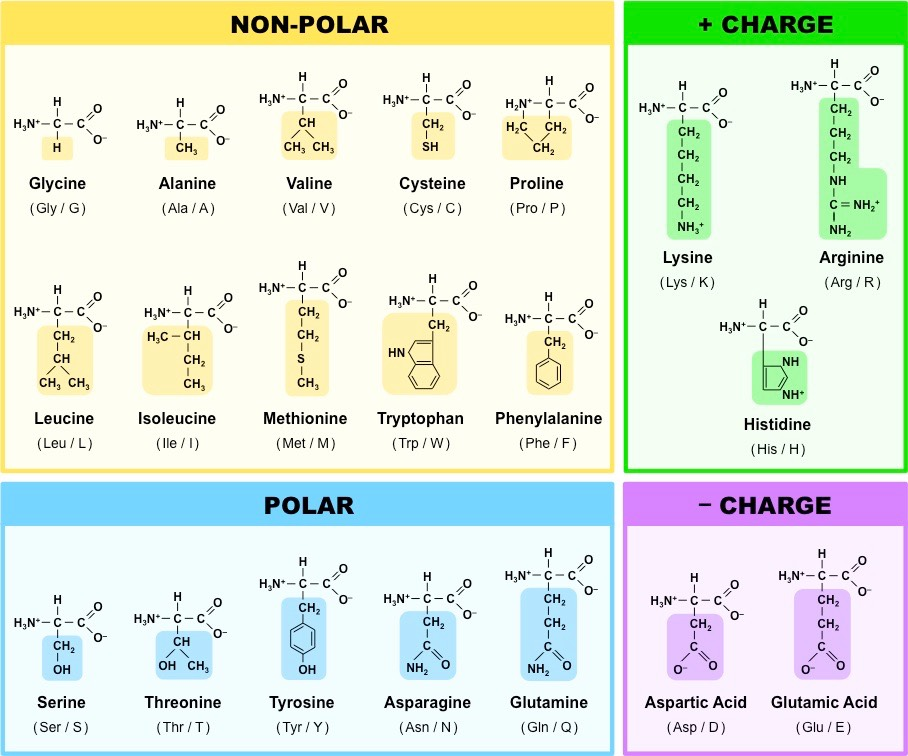
\includegraphics[scale=0.4]{images/aminoacid-tipi.jpeg}
	\caption{I 20 amminoacidi universali. Fonte: \cite{aminoacidTipi}}
	\label{fig:amminoacidi-tipi}
\end{figure}

\clearpage